\subsubsection{Ion balance test}
\label{sec.tests.ionbalance}

The one-zone collapse problem, described in \S\ref{sec.tests.1-zone},
is a good test of the chemistry solver at low temperatures where it is
difficult to calculate an analytical solution for the equilibrium
fraction of each species.  However, for a gas of primordial composition
at high temperatures, a simple analytical solution exists for the
ionization balance of H and He species.  The equations balancing
ionization and recombination for all ions of H and He result in six
equations with six unknowns \citep[e.g.,][]{1996ApJS..105...19K}, are
given by
\begin{equation} \label{eq:eqnHI}
n_{\rm HI} = \frac{n_{\rm H} \alpha_{\rm HII}}{\alpha_{\rm HII}
+ \Gamma_{\rm eHI} + \Gamma_{\gamma \rm HI} / n_{\rm e}},
\end{equation}
\begin{equation}
n_{\rm HII} = n_{\rm H} - n_{\rm HI},
\end{equation}
\begin{equation}
n_{\rm HeII} = \frac{n_{\rm He}}{1 + \frac{\alpha_{\rm HeII}
+ \alpha_{\rm d}}{\Gamma_{\rm eHeI} + \Gamma_{\gamma \rm HeI} / n_{\rm
e}} + \frac{\Gamma_{\rm eHeII} + \Gamma_{\gamma \rm HeII} / n_{\rm
e}}{\alpha_{\rm HeIII}}},
\end{equation}
\begin{equation}
n_{\rm HeI} = n_{\rm HeII} \frac{\alpha_{\rm HeII} + \alpha_{\rm
d}}{\Gamma_{\rm eHeI} + \Gamma_{\gamma \rm HeI} / n_{\rm e}},
\end{equation}
\begin{equation}
n_{\rm HeIII} = n_{\rm HeII} \frac{\Gamma_{\rm eHeII}
+ \Gamma_{\rm \gamma \rm HeII} / n_{\rm e}}{\alpha_{\rm HeIII}},
\end{equation}
\begin{equation} \label{eq:eqne}
n_{\rm e} = n_{\rm HII} + n_{\rm HeII} + 2 n_{\rm HeIII},
\end{equation}
where $n_{\rm H}$ and $n_{\rm He}$ are the total number densities of
all H and He ions, $\alpha_{\rm i}$ is the recombination rate of
species i, and $\Gamma_{ij}$ is the ionization rate of species j by
i, where i is either an electron for collisional ionization or a
photon for photo-ionization.

In this test, we initialize a one-dimension grid at a constant number
density of 1 cm$^{-3}$ with smoothly varying temperature from 10$^{4}$
K to 10$^{9}$ K.  The gas is initially fully ionized and we then
iterate the chemistry equations without allowing the gas to cool until
convergence is reached.  In Figure \ref{fig.eq_test}, we show the
equilibrium ionization fractions for H and He ions and the resulting
cooling rate.  We assume no photo-ionization for this test.  
The results from this test are shown by the solid lines 
with the analytic solution decribed by 
Equations \ref{eq:eqnHI}--\ref{eq:eqne} using the rate equations 
in \enzo, referenced in \S\ref{sec.num.chemistry}, overplotted with
the dashed lines and an analytical solution using the rates 
of \citet{1992ApJS...78..341C}, shown by the dotted lines.  As can be
seen, the \enzo\ chemistry solver and corresponding analytical
solution are in perfect agreement.  The results largely agree with
those of \citet{1992ApJS...78..341C}, save for HI, HeI, and HeII at
high temperatures, where their ion fractions are quite low.  The
slightly higher abundance of HeI in \citet{1992ApJS...78..341C}
results in a higher cooling rate by about a factor of 2 near $T \sim
10^{5}$ K due to the enhanced collisional excitation cooling of HeI.

\begin{figure}
  \begin{center}
    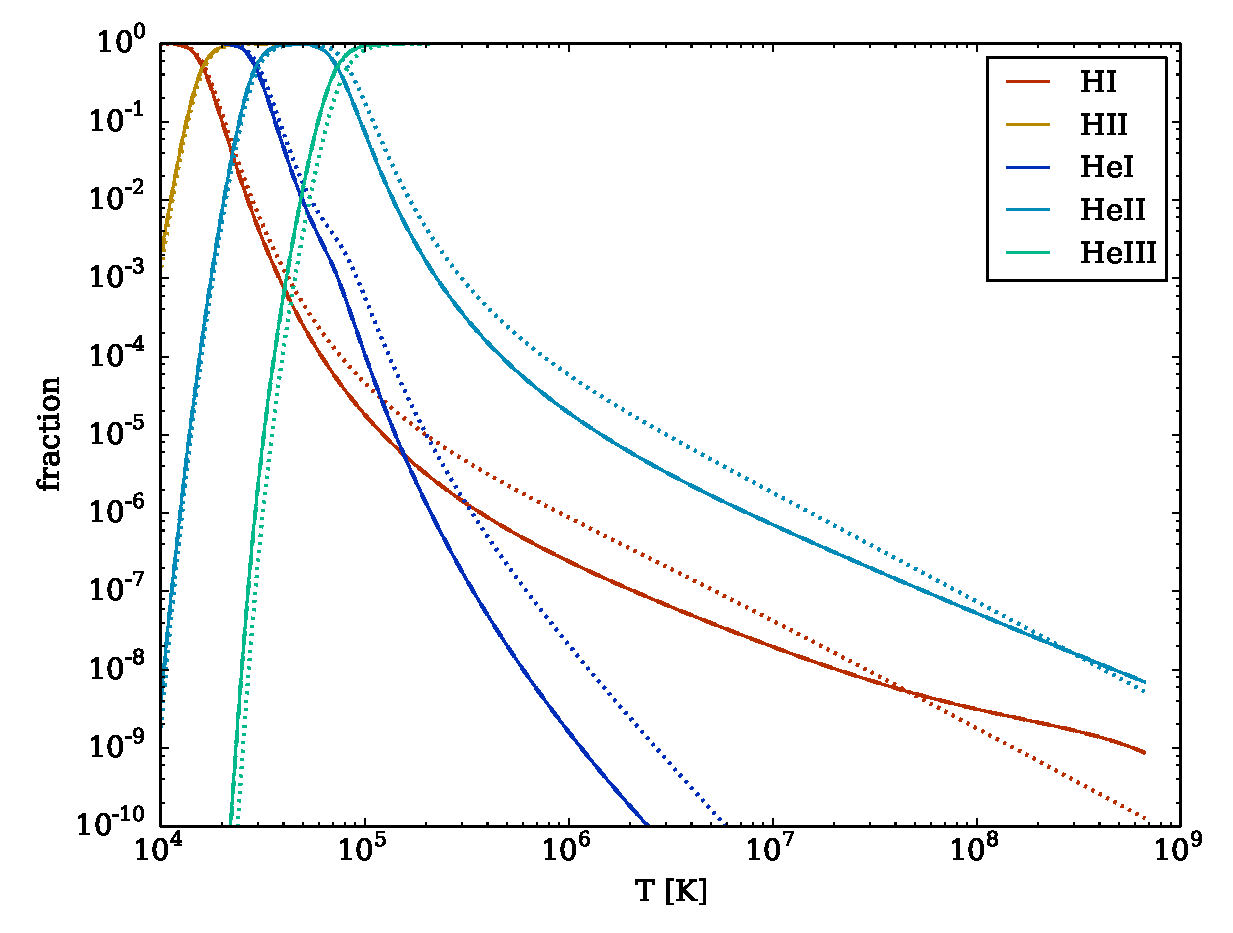
\includegraphics[width=0.49\textwidth]{figures/eq_ionization.eps}
    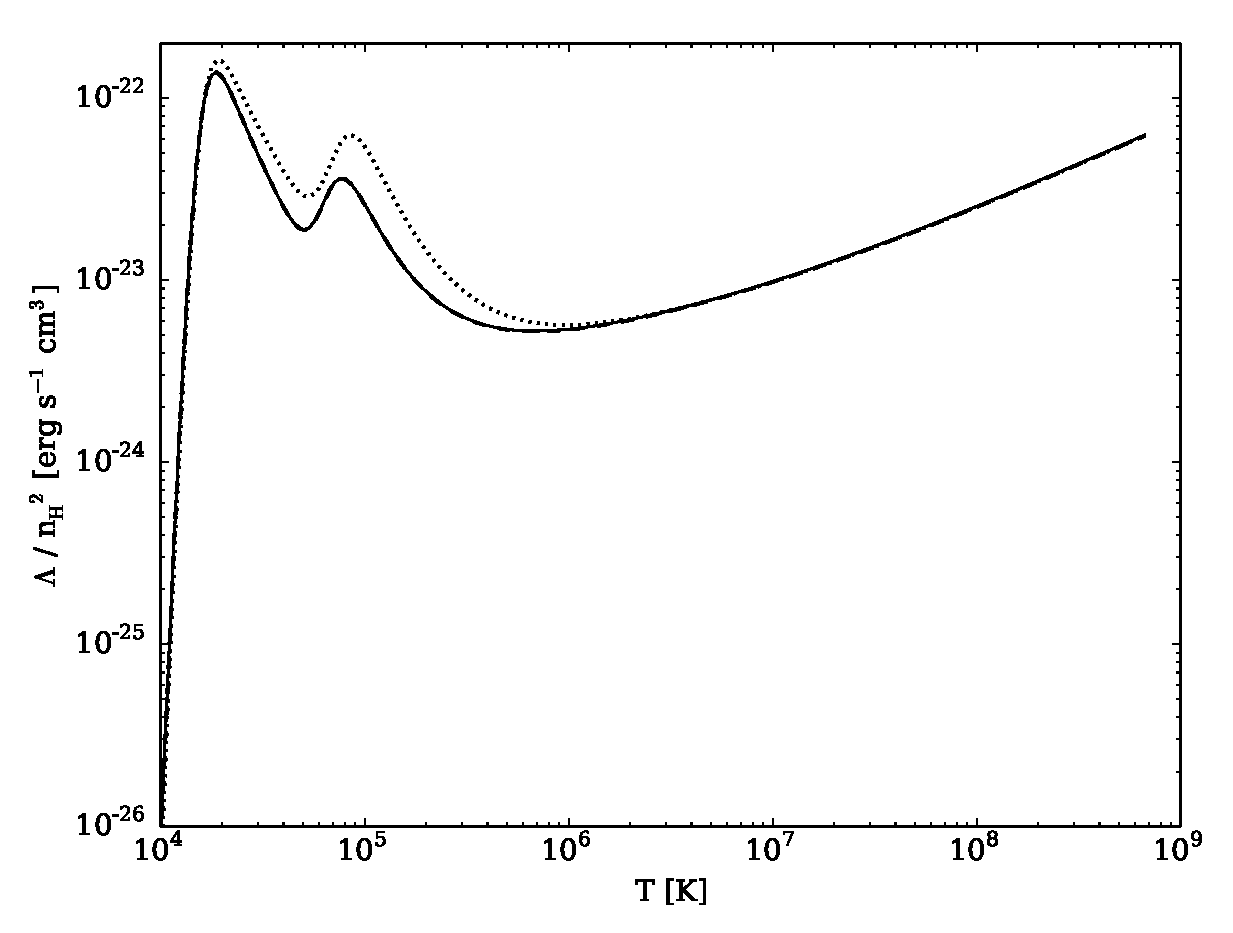
\includegraphics[width=0.49\textwidth]{figures/eq_cooling.eps}
  \end{center}
  \caption{Results of the ionization balance test
    (\S\ref{sec.tests.ionbalance}) calculating the equilibrium ionization
    balance (left) and resulting cooling rate (right) of a primordial
    gas with no incident photo-ionizing radiation.  Solid lines show
    the results of iterating the \enzo\ chemistry solver to
    convergence.  Dashed lines (directly underneath the solid lines)
    show the analytical solution using the same rates.  Dotted 
    lines show the analytical solution using the rates
    of \citet{1992ApJS...78..341C}.}
  \label{fig.eq_test}
\end{figure}
